\chapter{Dữ liệu không gian địa lý}
\label{ch:M6L1LessonNotes}

\section*{Lesson Notes}

MODULE 6 \textbar{} BÀI 1

{\small
\begin{longtable}[]{@{}
  >{\raggedright\arraybackslash}p{(\columnwidth - 2\tabcolsep) * \real{0.5000}}
  >{\raggedright\arraybackslash}p{(\columnwidth - 2\tabcolsep) * \real{0.5000}}@{}}
\toprule\noalign{}
\endhead
\bottomrule\noalign{}
\endlastfoot
\textbf{Thời gian đọc} & 60 phút \\
\textbf{Kiến thức nền} & Python cơ bản \\
\textbf{Từ khóa} & Dữ liệu không gian địa lý, dữ liệu raster, dữ liệu vector, GIS, CRS \\
& \\
& \\
\end{longtable}
}

\section{Giới thiệu}

Trong bài học này, chúng ta sẽ làm quen với dữ liệu không gian địa lý (geospatial data). Loại dữ liệu này được gắn thông tin vị trí dưới dạng một hệ tọa độ. Chúng ta sẽ đi qua các khái niệm cơ bản về dữ liệu không gian địa lý, sau đó minh họa cách dùng Python để xử lý loại dữ liệu này phục vụ cho phân tích tiếp theo. Kiến thức học được từ bài học này cũng sẽ giúp ích cho các bài học sắp tới của module về ảnh vệ tinh và dữ liệu khí hậu.

\section{Dữ liệu không gian địa lý}

\subsection{Dữ liệu không gian địa lý là gì?}

\textbf{Dữ liệu không gian địa lý} (Geospatial Data) là một loại tập dữ liệu chứa thông tin về các đặc trưng (feature) trên bề mặt Trái Đất. Đặc trưng là gì? Những sự vật hoặc sự kiện mà chúng ta có thể quan sát được trên bề mặt Trái Đất được gọi là các đặc trưng. Ví dụ, một cái cây, một tòa nhà, một con đường và một dòng sông là những ví dụ về đặc trưng. Đây là các đặc trưng tĩnh, không di chuyển hoặc thay đổi quá nhanh. Đặc trưng cũng có thể mang tính động, chẳng hạn như lộ trình di chuyển của một chiếc xe hoặc đường đi của một cơn bão.

Thông tin về đặc trưng trong một tập dữ liệu không gian địa lý gồm hai thành phần: \textbf{vị trí của đặc trưng} và \textbf{thuộc tính của đặc trưng}.

~~~~~~\textbf{Vị trí của đặc trưng} cho biết đặc trưng này nằm ở đâu trong một hệ tọa độ trên bề mặt Trái Đất. Tùy thuộc vào kiểu dữ liệu trong tập dữ liệu không gian địa lý, có nhiều phương pháp khác nhau để biểu diễn thông tin về vị trí của đặc trưng. Chúng ta sẽ thảo luận thêm về vấn đề này ở phần sau của bài học.

~~~~~~\textbf{Thuộc tính của đặc trưng} cho biết các thông tin khác không liên quan đến định vị, chẳng hạn như chiều cao của một tòa nhà, năm xây dựng, v.v. Một ví dụ khác là tốc độ và áp suất của một cơn bão tại một thời điểm nhất định.

Khi thảo luận về vị trí của đặc trưng, chúng ta đã nói đến việc biểu diễn một vị trí trong hệ tọa độ của bề mặt Trái Đất. Trong phần tiếp theo, chúng ta sẽ tìm hiểu thêm về các hệ tọa độ được sử dụng trong dữ liệu không gian địa lý.

\subsection{Dữ liệu không gian địa lý trong phân tích tài chính}

Trong những năm gần đây, việc áp dụng dữ liệu không gian địa lý (geospatial data) vào phân tích tài chính ngày càng phổ biến. Dữ liệu không gian địa lý có thể cung cấp nhiều khía cạnh thông tin về các hoạt động tài chính mà dữ liệu tài chính truyền thống không thể cung cấp. Dữ liệu không gian địa lý liên kết các kết quả kinh tế, sự di chuyển của con người hoặc vật thể, và sự thay đổi của môi trường tự nhiên với nhau. Dưới đây là một số ví dụ về cách áp dụng dữ liệu không gian địa lý trong phân tích tài chính.

~~~~~~\textbf{Hiểu rõ hơn về sự di chuyển của con người và vật thể}

~~~~~~Dữ liệu không gian địa lý giúp hiểu sâu hơn về sự di chuyển của cả con người lẫn vật thể. Chẳng hạn, bằng cách nắm được tần suất và thời điểm khách hàng đi bộ ghé qua một cửa hàng bán lẻ, các nhà phân tích tài chính có thể dự báo doanh số và đưa ra các quyết định sáng suốt về hiệu quả hoạt động của công ty.

~~~~~~\textbf{Đánh giá rủi ro tín dụng} Các tổ chức tài chính có thể sử dụng dữ liệu không gian địa lý để đánh giá rủi ro khi bảo lãnh một khoản vay bất động sản thương mại. Dữ liệu này có thể phân tích lịch sử trả nợ của các bất động sản thương mại lân cận.

~~~~~~\textbf{Lựa chọn vị trí chi nhánh ngân hàng} Bằng cách phân tích sự di chuyển và các tuyến đường mua sắm của cư dân trong một cộng đồng, ngân hàng có thể xác định vị trí tối ưu cho chi nhánh, sao cho giao cắt với tuyến đường đi lại của đa số cư dân.

\section{Hệ tham chiếu tọa độ}

\textbf{Hệ tham chiếu tọa độ (coordinate reference system, CRS)} là một hệ tọa độ dùng để mô tả thông tin vị trí trên bề mặt Trái Đất (Awati, 2022). Có nhiều khung hệ thống CRS có thể sử dụng, nhưng cách tiếp cận phổ biến nhất là dùng vĩ độ và kinh độ để tạo thành một hệ lưới trên bề mặt Trái Đất.

~~~~~~Các đường \textbf{vĩ độ (latitude)} là những đường ngang vắt qua Trái Đất, cho biết một vị trí cách xích đạo bao xa theo hướng bắc và nam. Đường vĩ độ 0 độ nằm tại xích đạo. Nó chia Trái Đất thành Bắc bán cầu phía trên xích đạo và Nam bán cầu phía dưới xích đạo.

~~~~~~Các đường \textbf{kinh độ (longitude)} là những đường dọc vắt qua Trái Đất, cho biết một vị trí cách kinh tuyến gốc bao xa theo hướng tây và đông. Đường kinh độ 0 độ nằm tại kinh tuyến gốc. Nó chia Trái Đất thành Đông bán cầu và Tây bán cầu. Hình 1 minh họa hệ tọa độ này.

\textbf{Hình 1. Hệ tọa độ vĩ độ và kinh độ của Trái Đất}

\begin{figure}[H]
\centering
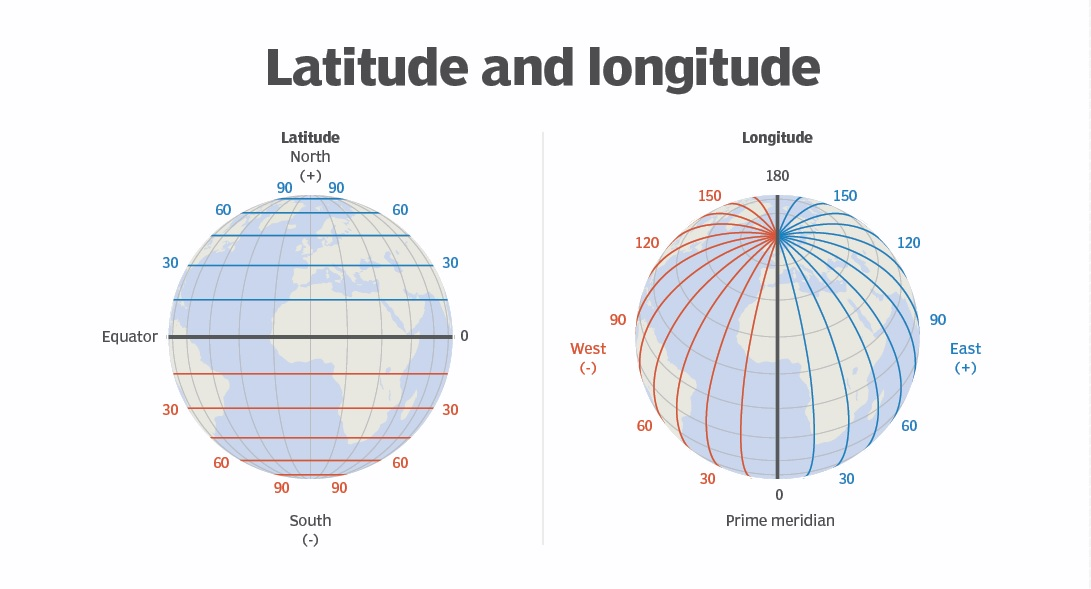
\includegraphics[width=0.85\linewidth]{gfx/m6l1_img002.jpeg}
\par\smallskip{\small \textbf{Hình:} Hệ tham chiếu tọa độ vĩ độ -- kinh độ. Nguồn: TechTarget.}
\end{figure}

\emph{Nguồn: TechTarget}

Khi xác định một vị trí trên CRS, quy ước chung là ghi vĩ độ trước, rồi đến kinh độ, theo dạng (vĩ độ, kinh độ). Có hai cách biểu diễn thông tin vĩ độ-kinh độ. Cách thứ nhất là độ, phút, giây (DMS). Ví dụ, tọa độ của New York theo DMS là (40° 43\textquotesingle{} 50.1960\textquotesingle\textquotesingle{} N, 73° 56\textquotesingle{} 6.8712\textquotesingle\textquotesingle{} W). Ký hiệu ° biểu thị độ, \textquotesingle{} biểu thị phút và \textquotesingle\textquotesingle{} biểu thị giây. Cách thứ hai là độ thập phân (DD). Tọa độ của New York theo DD là (40.730610, -73.935242).

DMS và DD có hai khác biệt chính. Khác biệt thứ nhất là DMS và DD dùng các ký hiệu khác nhau để biểu thị thông tin hướng của một vị trí. DMS dùng chữ cái để mô tả vị trí nằm ở bán cầu nào (N so với S; W so với E), còn DD dùng dấu + và - để mô tả bán cầu. Trong phương pháp DMS, tọa độ hướng của New York là (N, W). Trong phương pháp DD, tọa độ hướng của New York là (+,-). Chúng ta có thể dùng Hình 1 để hiểu cách phương pháp DD gán dấu +/-. Ở phần bên trái của hình, ta thấy nếu một vị trí nằm ở Bắc bán cầu thì dấu của vĩ độ là +; nếu vị trí nằm ở phía nam thì dấu của vĩ độ là -. Khái niệm này cũng áp dụng tương tự cho kinh độ.

Khác biệt thứ hai là DMS tính bằng độ, phút, giây còn DD tính bằng số thập phân. Chúng ta có thể dễ dàng chuyển đổi giữa hai phương pháp. Để chuyển từ DMS sang DD, trước tiên ta giữ nguyên số độ. Sau đó, ta chia số phút cho 60 và chia số giây cho 3600. Tiếp theo, ta cộng kết quả của hai phép chia này rồi cộng vào số độ. Con số cuối cùng chính là giá trị theo DD. Đôi khi, bán cầu của dữ liệu được chỉ ra bởi tên biến hoặc tiêu đề cột, và giá trị của các điểm dữ liệu trong bảng đều là số dương. Trong trường hợp này, chúng ta cần điều chỉnh thủ công giá trị của các điểm dữ liệu để biểu diễn đúng vị trí bán cầu theo phương pháp DD.

Trong Python, chúng ta sẽ dùng phương pháp DD để biểu diễn thông tin tọa độ. Bạn có thể dễ dàng tìm tọa độ DD của một địa điểm trên Google Maps.

\section{Các loại dữ liệu không gian địa lý}

Ở phần trước, chúng ta đã giới thiệu hệ tham chiếu tọa độ (CRS) kinh độ - vĩ độ. Trong phần về vị trí của đặc trưng, chúng ta đã nói rằng các loại dữ liệu địa lý khác nhau sẽ dùng những phương pháp khác nhau để biểu diễn thông tin vị trí. Có hai loại dữ liệu địa lý chính: dữ liệu raster và dữ liệu vector.

~~~~~~\textbf{Dữ liệu raster} chia một đặc trưng thành một hệ thống lưới. Mỗi ô lưới được gọi là một điểm ảnh (pixel) hoặc một ô (cell). Dữ liệu raster lưu trữ các thuộc tính của đặc trưng dựa trên từng điểm ảnh. Trong bài học về ảnh vệ tinh, chúng ta sẽ bàn kỹ hơn về dữ liệu raster.

~~~~~~\textbf{Dữ liệu vector} lưu trữ các thuộc tính của đặc trưng dựa trên hình dạng của đặc trưng. Một đặc trưng có thể có dạng điểm, dạng đường hoặc dạng đa giác. Trong bài học này, chúng ta sẽ tập trung vào dữ liệu vector.

Trước khi chuyển sang chủ đề tiếp theo về dữ liệu vector, hãy xem Hình 2 để hình dung trực quan sự khác biệt giữa hai loại dữ liệu địa lý này.

\textbf{Hình 2. Dữ liệu vector và dữ liệu raster}

\begin{figure}[H]
\centering
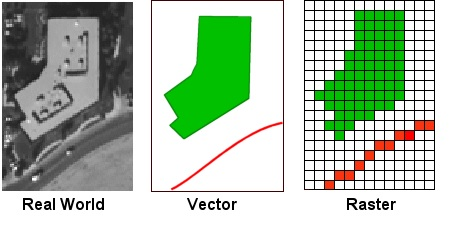
\includegraphics[width=0.85\linewidth]{gfx/m6l1_img003.jpeg}
\par\smallskip{\small \textbf{Hình:} Dữ liệu vector và dữ liệu raster biểu diễn thế giới thực. Nguồn: CUNY Hunter.}
\end{figure}

\emph{Nguồn: CUNY Hunter}

\section{Dữ liệu vector}

Ở phần trước, chúng ta đã trình bày cách biểu diễn một vị trí bằng CRS. Cho đến nay, ta mới chỉ đề cập đến vị trí điểm, tức là một chấm trên hệ tọa độ vĩ độ - kinh độ. Ngoài hình dạng điểm, chúng ta còn có thể đưa vào các hình dạng đường và hình dạng đa giác cùng với CRS. Hình 3 minh họa ví dụ về hình dạng điểm, hình dạng đường và hình dạng đa giác.

\textbf{Hình 3. Các hình dạng điểm, đường và đa giác}

\begin{figure}[H]
\centering
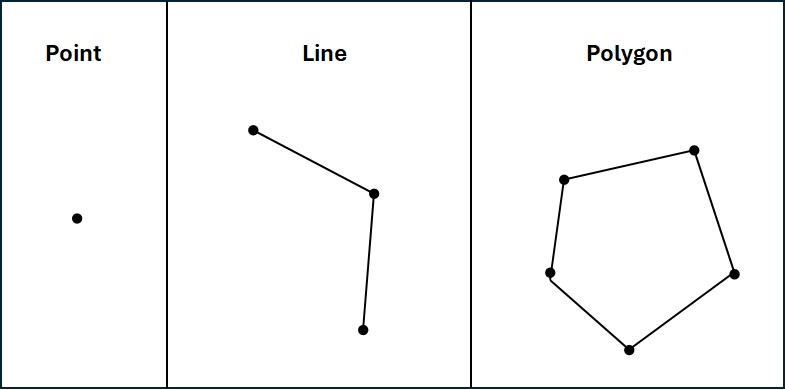
\includegraphics[width=0.85\linewidth]{gfx/m6l1_img001.jpeg}
\par\smallskip{\small \textbf{Hình:} Dữ liệu vector: điểm, đường và đa giác.}
\end{figure}

Ba hình dạng trên trong Hình 3 đều được cấu thành từ các điểm và các đường. Các điểm này được gọi là đỉnh (vertex). Vị trí của mỗi đỉnh có thể được biểu diễn bằng một cặp tọa độ vĩ độ - kinh độ. Nhờ có thông tin về hình dạng và thông tin về tọa độ của các đỉnh, chúng ta có thể xác định vị trí không gian địa lý của một đặc trưng trên hệ tọa độ vĩ độ - kinh độ. Trong dữ liệu vector, chúng ta lưu trữ thông tin hình dạng và thông tin tọa độ trong một biến gọi là \textbf{geometry}. Chính biến geometry này làm cho dữ liệu không gian địa lý khác biệt với dữ liệu dạng bảng truyền thống. Về định dạng dữ liệu không gian địa lý vector, có hai định dạng phổ biến: \textbf{GeoJSON} và \textbf{Shapefile}. Các tài liệu đọc bắt buộc sẽ giới thiệu rất ngắn gọn về hai định dạng dữ liệu này.

\section{Nguồn dữ liệu không gian địa lý và phần mềm phân tích}

Có nhiều cách để thu thập dữ liệu không gian địa lý. Một số nguồn thu thập dữ liệu gồm Hệ thống định vị toàn cầu (GPS), thiết bị đeo, điện thoại di động, viễn thám (vệ tinh) và Internet vạn vật (IoT), cùng nhiều nguồn khác.

Sau khi có dữ liệu không gian địa lý, các nhà nghiên cứu thường dùng \textbf{hệ thống thông tin địa lý (GIS)} để đọc và phân tích dữ liệu. Có nhiều GIS phổ biến, trả phí hoặc miễn phí, như ArcGIS hoặc QGIS. Các phần mềm này thường có sẵn các hàm đọc nhiều loại dữ liệu không gian địa lý khác nhau và các hàm trực quan hóa để trình bày dữ liệu.

\section{Ứng dụng của dữ liệu không gian địa lý}

Trong phần này, chúng ta sẽ sử dụng Python để minh họa cách lấy dữ liệu không gian địa lý từ nguồn dữ liệu trực tuyến, làm sạch dữ liệu để sẵn sàng cho phân tích và trực quan hóa dữ liệu.

Chúng ta sẽ lấy đường đi của bão Irene dọc theo bờ biển phía đông Hoa Kỳ làm ví dụ. Vào cuối tháng 8 năm 2011, bão Irene đã gây thiệt hại nghiêm trọng cho khu vực này của Hoa Kỳ. Chẳng hạn, khu vực hạ Manhattan của thành phố New York bị mất điện trong một tuần do cơn bão.

Trong ứng dụng này, chúng ta sẽ lấy dữ liệu về đường đi và sức gió của cơn bão từ Trung tâm Bão Quốc gia (National Hurricane Center - NHC) thuộc Cơ quan Quản lý Khí quyển và Đại dương Quốc gia Hoa Kỳ (National Oceanic and Atmospheric Administration - NOAA). Chúng ta sẽ lấy dữ liệu và vẽ đường đi của cơn bão lên bản đồ. Trong phần minh họa này, chúng ta cũng sẽ trình bày cách chồng các thông tin khác nhau lên bản đồ. Chúng ta sẽ chồng ranh giới các bang của Hoa Kỳ lên bản đồ để cho thấy những bang nào chịu ảnh hưởng của cơn bão này.

Gói Python chính dùng để phân tích dữ liệu không gian địa lý là geopandas. Geopandas là phiên bản dữ liệu không gian địa lý của pandas. Gói này có thể xử lý nhiều loại dữ liệu không gian địa lý mà chúng ta đã đề cập ở các phần trước. Sau đó, chúng ta sẽ dùng gói folium để trực quan hóa đường đi của cơn bão. Chúng ta bắt đầu thôi.

\subsection{Tải các gói Python}

Chúng ta sẽ cần một số gói cho phần minh họa này.

\begin{lstlisting}[language=Python,escapeinside={(*@}{@*)}]
!pip install fiona
\end{lstlisting}

\begin{lstlisting}[language=Python,escapeinside={(*@}{@*)}]
!pip install geopandas
\end{lstlisting}

\begin{lstlisting}[language=Python,escapeinside={(*@}{@*)}]
pip install install-jdk
\end{lstlisting}

\begin{lstlisting}[language=Python,escapeinside={(*@}{@*)}]
import jdk
from jdk.enums import OperatingSystem, Architecture

jdk.install('11', operating_system=OperatingSystem.LINUX)
\end{lstlisting}

Output:

\begin{lstlisting}[escapeinside={(*@}{@*)}]
'/root/.jdk/jdk-11.0.25+9'
\end{lstlisting}

\begin{lstlisting}[language=Python,escapeinside={(*@}{@*)}]
import os
jdk_version = 'jdk-11.0.25+9' #change with your version 
os.environ['JAVA_HOME'] = '/root/.jdk/jdk-11.0.25+9'
os.environ['PATH'] = f"{os.environ.get('PATH')}:{os.environ.get('JAVA_HOME')}/bin"
\end{lstlisting}

\begin{lstlisting}[language=Python,escapeinside={(*@}{@*)}]
# (*@Nhập@*) (*@các@*) (*@gói@*) cho (*@ứng@*) (*@dụng@*) (*@này@*)
# pandas (*@dùng@*) (*@để@*) (*@xử@*) (*@lý@*) dataframe (*@và@*) geopandas (*@dùng@*) (*@để@*) (*@xử@*) (*@lý@*) geodataframe
# fiona (*@dùng@*) (*@để@*) (*@đọc@*) (*@hoặc@*) ghi (*@nhiều@*) (*@định@*) (*@dạng@*) (*@dữ@*) (*@liệu@*) (*@không@*) gian (*@địa@*) (*@lý@*)
# urllib (*@dùng@*) (*@để@*) (*@lấy@*) (*@dữ@*) (*@liệu@*) (*@trên@*) internet (*@bằng@*) url
# zipfile (*@dùng@*) (*@để@*) (*@giải@*) (*@nén@*) (*@tệp@*) zip
import os
import pandas as pd
import geopandas as gpd
import fiona
import urllib.request
import zipfile
\end{lstlisting}

\subsection{Dữ liệu về cơn bão Irene}

Dữ liệu về đường đi của cơn bão nằm trong một tệp PDF. Do đó, chúng ta cần cài đặt gói tabula để xử lý các tệp PDF.

\begin{lstlisting}[language=Python,escapeinside={(*@}{@*)}]
pip install tabula-py
\end{lstlisting}

\begin{lstlisting}[language=Python,escapeinside={(*@}{@*)}]
# Import tabula package for PDF handling
import tabula
\end{lstlisting}

Tiếp theo, hãy lấy tệp PDF từ trang web của Trung tâm Bão Quốc gia Hoa Kỳ (National Hurricane Center, NHC).

\begin{lstlisting}[language=Python,escapeinside={(*@}{@*)}]
# Retrieve PDF file from NHC website
url = "https://www.nhc.noaa.gov/data/tcr/AL092011_Irene.pdf"

irene_pdf, _ = urllib.request.urlretrieve(url)
\end{lstlisting}

Sau đó, chúng ta sẽ dùng một phương thức của gói tabula để chuyển tệp PDF thành tệp csv.

\begin{lstlisting}[language=Python,escapeinside={(*@}{@*)}]
# Convert PDF file to csv file, and then a pandas dataframe
tabula.convert_into(irene_pdf, "irene.csv", output_format="csv", stream=True, pages = 9)
irene_1 = pd.read_csv("irene.csv")
irene_1
\end{lstlisting}

Từ kết quả của đoạn mã trước, ta thấy hàng thứ hai không chứa giá trị dữ liệu. Đó là các đơn vị đo lường/thông tin của từng biến. Ví dụ, đơn vị đo của tốc độ gió là hải lý/giờ (knot, kt). Ngoài ra, hàng cuối cùng cũng không có giá trị dữ liệu nào. Chúng ta sẽ loại bỏ hai hàng này.

\begin{lstlisting}[language=Python,escapeinside={(*@}{@*)}]
# Drop rows with measurement units or no data values
irene_1.drop([0,40], inplace = True)
irene_1
\end{lstlisting}

Tiếp theo, hãy chuyển các biến số sang kiểu số thực (float).

\begin{lstlisting}[language=Python,escapeinside={(*@}{@*)}]
# Correct data types for numeric variables
convert_dict = {'Date/Time': str,
                'Latitude': float,
                'Longitude': float,
                'Pressure': float,
                'Wind Speed': float
                }

irene_1 = irene_1.astype(convert_dict)
print(irene_1.dtypes)
\end{lstlisting}

Kết quả:

\begin{lstlisting}[escapeinside={(*@}{@*)}]
Date/Time      object
Latitude      float64
Longitude     float64
Pressure      float64
Wind Speed    float64
Unnamed: 5     object
dtype: object
\end{lstlisting}

\subsection{Tạo biến ngày-giờ}

Tiếp theo, ta thấy biến ngày/giờ không chứa thông tin về tháng và năm. Do đó, chúng ta sẽ tạo một biến ngày/giờ mới để cung cấp thông tin ngày/giờ đầy đủ.

\begin{lstlisting}[language=Python,escapeinside={(*@}{@*)}]
# Create a new Date Time variable to contain month and year information
irene_1[["Date","Time"]] = irene_1["Date/Time"].str.split(" / ", expand = True)
irene_1["Date_Time"] = "08/" + irene_1["Date"] + "/2011/" + irene_1["Time"]
irene_1.set_index("Date_Time")
irene_1
\end{lstlisting}

\subsection{Đảm bảo dữ liệu không gian địa lý chính xác}

Chúng ta cũng nhận thấy rằng các giá trị kinh độ trong bộ dữ liệu đều là số dương. Tuy nhiên, hướng của kinh độ là "W" (Tây). Dựa trên Hình 1 ở mục 3, các số liệu kinh độ lẽ ra phải là số âm. Do đó, chúng ta cần thêm dấu âm vào trước tất cả các giá trị của biến kinh độ để phản ánh đúng vị trí.

\begin{lstlisting}[language=Python,escapeinside={(*@}{@*)}]
# Adjust Longitude value to correctly reflect the geolocation
irene_1['Longitude'] = 0 - irene_1['Longitude']
\end{lstlisting}

\begin{lstlisting}[language=Python,escapeinside={(*@}{@*)}]
# Select the variables we are interest for next steps
irene_2 = irene_1[["Date_Time","Longitude","Latitude","Wind Speed"]]
\end{lstlisting}

\subsection{Chuyển đổi sang Geodataframe}

Bây giờ chúng ta đã có một dataframe hoàn chỉnh cho đường đi của bão Irene. Để chuyển dataframe này thành dataframe không gian địa lý, chúng ta cần tạo một biến hình học (geometry), như đã giải thích ở phần trước. Chúng ta sẽ dùng một phương thức của geopandas để tạo biến này. Một trong các tham số trong đoạn mã dưới đây là "EPSG:4326", là mã định danh của hệ kinh độ - vĩ độ mà chúng ta đã quen thuộc. Hãy nhớ rằng có nhiều hệ tham chiếu tọa độ (CRS) khác nhau, nhưng chúng ta sẽ tiếp tục với hệ được sử dụng phổ biến này.

\begin{lstlisting}[language=Python,escapeinside={(*@}{@*)}]
# (*@Tạo@*) (*@biến@*) (*@vị@*) (*@trí@*) (*@địa@*) (*@lý@*)
geometry = gpd.points_from_xy(irene_2.Longitude, irene_2.Latitude, crs="EPSG:4326")
\end{lstlisting}

Bây giờ hãy chuyển pandas dataframe hiện tại thành geodataframe.

\begin{lstlisting}[language=Python,escapeinside={(*@}{@*)}]
# (*@Chuyển@*) dataframe (*@hiện@*) (*@tại@*) (*@thành@*) geodataframe (*@với@*) (*@biến@*) geometry
irene_3 = gpd.GeoDataFrame(
    irene_2, geometry=geometry, crs="EPSG:4326"
)
\end{lstlisting}

Tuyệt vời! Bây giờ chúng ta đã có một geodataframe. Hãy xem năm dòng đầu tiên của dataframe này.

\begin{lstlisting}[language=Python,escapeinside={(*@}{@*)}]
irene_3.head()
\end{lstlisting}

Output:

\begin{lstlisting}[escapeinside={(*@}{@*)}]
         Date_Time  Longitude  Latitude  Wind Speed            geometry
1  08/21/2011/0000      -59.0      15.0        45.0      POINT (-59 15)
2  08/21/2011/0600      -60.6      16.0        45.0    POINT (-60.6 16)
3  08/21/2011/1200      -62.2      16.8        45.0  POINT (-62.2 16.8)
4  08/21/2011/1800      -63.7      17.5        50.0  POINT (-63.7 17.5)
5  08/22/2011/0000      -65.0      17.9        60.0    POINT (-65 17.9)
\end{lstlisting}

Trong biến geometry của geodataframe ở trên, chúng ta có các hình dạng điểm và cặp tọa độ của chúng trên bản đồ. Hãy xác nhận kiểu của dataframe mới này.

\begin{lstlisting}[language=Python,escapeinside={(*@}{@*)}]
type(irene_3)
\end{lstlisting}

Output:

\begin{lstlisting}[escapeinside={(*@}{@*)}]
geopandas.geodataframe.GeoDataFrame
\end{lstlisting}

Và hãy kiểm tra biến geometry của chúng ta.

\begin{lstlisting}[language=Python,escapeinside={(*@}{@*)}]
type(irene_3['geometry'])
\end{lstlisting}

Output:

\begin{lstlisting}[escapeinside={(*@}{@*)}]
geopandas.geoseries.GeoSeries
\end{lstlisting}

Về cơ bản, geodataframe hoạt động giống như pandas dataframe. Do đó, chúng ta có thể áp dụng các phương thức và phân tích tương tự của pandas cho geopandas. Sau đây là một ví dụ.

\begin{lstlisting}[language=Python,escapeinside={(*@}{@*)}]
print("Mean wind speed of Hurricane Irene is {} knots and it can go up to {} knots maximum".format(round(irene_2['Wind Speed'].mean(),4),
                                                                                         irene_2['Wind Speed'].max())+".")
\end{lstlisting}

Output:

\begin{lstlisting}[escapeinside={(*@}{@*)}]
Mean wind speed of Hurricane Irene is 69.6154 knots and it can go up to 105.0 knots maximum.
\end{lstlisting}

\subsection{Dữ liệu ranh giới các bang của Hoa Kỳ}

Trước khi vẽ đường đi của bão Irene lên bản đồ, chúng ta muốn thêm một lớp ranh giới các bang của Hoa Kỳ vào bản đồ. Khi trực quan hóa ranh giới các bang cùng với đường đi của bão Irene, chúng ta có thể biết những bang nào bị ảnh hưởng bởi cơn bão này. Chúng ta sẽ lấy tệp ranh giới các bang từ trang web của Cục Điều tra Dân số Hoa Kỳ (United States Census Bureau). Đây là một shapefile được nén dạng zip. Trước tiên, chúng ta cần nhập một gói để giải nén tệp.

\begin{lstlisting}[language=Python,escapeinside={(*@}{@*)}]
# (*@Nhập@*) (*@gói@*) (*@giải@*) (*@nén@*) (*@tệp@*)
from zipfile import ZipFile
\end{lstlisting}

\begin{lstlisting}[language=Python,escapeinside={(*@}{@*)}]
# (*@Lấy@*) shapefile (*@các@*) bang (*@của@*) Hoa (*@Kỳ@*) (*@từ@*) United States Census Bureau
us_state_url = "	http://www2.census.gov/geo/tiger/TIGER2012/STATE/tl_2012_us_state.zip"

us_state_shape_zip, _ = urllib.request.urlretrieve(us_state_url)
\end{lstlisting}

\begin{lstlisting}[language=Python,escapeinside={(*@}{@*)}]
# (*@Giải@*) (*@nén@*) shapefile (*@và@*) (*@đặt@*) (*@tên@*) (*@mới@*) (*@là@*) "us_state_shape"
with ZipFile(us_state_shape_zip, 'r') as zObject:

    zObject.extractall("us_state_shape")
\end{lstlisting}

Sau khi giải nén tệp, chúng ta sẽ dùng phương thức read\_file của geopandas để đọc tệp này thành một geodataframe nhằm xử lý dữ liệu tiếp theo.

\begin{lstlisting}[language=Python,escapeinside={(*@}{@*)}]
# (*@Đọc@*) shapefile (*@vào@*) (*@một@*) geodataframe
us_state_shape_g = gpd.read_file("us_state_shape")
\end{lstlisting}

\begin{lstlisting}[language=Python,escapeinside={(*@}{@*)}]
# (*@Kiểm@*) tra (*@siêu@*) (*@dữ@*) (*@liệu@*) (*@của@*) geodataframe (*@mới@*)
us_state_shape_g.info()
\end{lstlisting}

Output:

\begin{lstlisting}[escapeinside={(*@}{@*)}]
<class 'geopandas.geodataframe.GeoDataFrame'>
RangeIndex: 56 entries, 0 to 55
Data columns (total 15 columns):
 #   Column    Non-Null Count  Dtype   
---  ------    --------------  -----   
 0   REGION    56 non-null     object  
 1   DIVISION  56 non-null     object  
 2   STATEFP   56 non-null     object  
 3   STATENS   56 non-null     object  
 4   GEOID     56 non-null     object  
 5   STUSPS    56 non-null     object  
 6   NAME      56 non-null     object  
 7   LSAD      56 non-null     object  
 8   MTFCC     56 non-null     object  
 9   FUNCSTAT  56 non-null     object  
 10  ALAND     56 non-null     int64   
 11  AWATER    56 non-null     int64   
 12  INTPTLAT  56 non-null     object  
 13  INTPTLON  56 non-null     object  
 14  geometry  56 non-null     geometry
dtypes: geometry(1), int64(2), object(12)
memory usage: 6.7+ KB
\end{lstlisting}

\begin{lstlisting}[language=Python,escapeinside={(*@}{@*)}]
# (*@Kiểm@*) tra (*@vài@*) (*@dòng@*) (*@đầu@*) (*@của@*) geodataframe (*@mới@*)
us_state_shape_g.head()
\end{lstlisting}

Output:

\begin{lstlisting}[escapeinside={(*@}{@*)}]
  REGION DIVISION STATEFP   STATENS GEOID STUSPS        NAME LSAD  MTFCC   
0      4        9      15  01779782    15     HI      Hawaii   00  G4000  \
1      3        7      05  00068085    05     AR    Arkansas   00  G4000   
2      4        8      35  00897535    35     NM  New Mexico   00  G4000   
3      4        8      30  00767982    30     MT     Montana   00  G4000   
4      1        2      36  01779796    36     NY    New York   00  G4000   

  FUNCSTAT         ALAND       AWATER     INTPTLAT      INTPTLON   
0        A   16634247483  11678744699  +19.8097670  -155.5061027  \
1        A  134772564356   2959210006  +34.8955256  -092.4446262   
2        A  314161109357    756438507  +34.4346843  -106.1316181   
3        A  376963571188   3868564895  +47.0511771  -109.6348174   
4        A  122057936950  19238848209  +42.9133974  -075.5962723   

                                            geometry  
0  MULTIPOLYGON (((-155.96333 19.08159, -155.9634...  
1  POLYGON ((-94.46025 34.53838, -94.46026 34.543...  
2  POLYGON ((-109.04616 34.57929, -109.04616 34.5...  
3  POLYGON ((-114.33289 46.66076, -114.33367 46.6...  
4  MULTIPOLYGON (((-79.64546 41.99886, -79.6498 4...
\end{lstlisting}

\subsection{Trực quan hóa dữ liệu không gian địa lý}

Bây giờ chúng ta đã có tệp về đường đi của bão Irene và tệp về ranh giới các bang của Hoa Kỳ. Cả hai đều ở dạng geodataframe. Chúng ta có thể đưa toàn bộ thông tin vào một bản đồ để trực quan hóa. Chúng ta sẽ dùng gói folium để vẽ bản đồ, rồi thêm ranh giới các bang của Hoa Kỳ và đường đi của cơn bão vào bản đồ.

\begin{lstlisting}[language=Python,escapeinside={(*@}{@*)}]
pip install folium
\end{lstlisting}

\begin{lstlisting}[language=Python,escapeinside={(*@}{@*)}]
# Import a mapping library
import folium
\end{lstlisting}

Tuyệt vời! Bây giờ là lúc đưa thông tin lên bản đồ.

\begin{lstlisting}[language=Python,escapeinside={(*@}{@*)}]
# (*@Vẽ@*) (*@đường@*) (*@đi@*) (*@của@*) (*@bão@*) Irene (*@và@*) (*@các@*) (*@thông@*) tin (*@khác@*) (*@lên@*) (*@bản@*) (*@đồ@*)

# (*@Đầu@*) (*@tiên@*), (*@tạo@*) (*@bản@*) (*@đồ@*) (*@nền@*)
map = folium.Map(location=[30,-102], zoom_start=4, control_scale=True)

# Sau (*@đó@*) (*@thêm@*) (*@lớp@*) (*@đầu@*) (*@tiên@*) (*@là@*) ranh (*@giới@*) (*@các@*) bang (*@của@*) Hoa (*@Kỳ@*) (*@vào@*) (*@bản@*) (*@đồ@*)
folium.GeoJson(us_state_shape_g).add_to(map)

# (*@Tiếp@*) theo (*@thêm@*) (*@đường@*) di (*@chuyển@*) (*@của@*) (*@cơn@*) (*@bão@*) (*@vào@*) (*@bản@*) (*@đồ@*). (*@Chúng@*) ta (*@dùng@*) (*@một@*) (*@chấm@*) (*@đỏ@*) (*@để@*) (*@biểu@*) (*@diễn@*) (*@vị@*) (*@trí@*) (*@của@*) (*@cơn@*) (*@bão@*) (*@tại@*) (*@một@*) (*@ngày@*)/(*@giờ@*) (*@cụ@*) (*@thể@*). Sau (*@đó@*) (*@thêm@*) (*@một@*) (*@hộp@*) (*@thông@*) tin (*@và@*) (*@một@*) (*@hộp@*) popup. (*@Nếu@*) di (*@chuột@*) (*@đến@*) (*@chấm@*) (*@đỏ@*), (*@bản@*) (*@đồ@*) (*@sẽ@*) (*@hiển@*) (*@thị@*) (*@ngày@*)/(*@giờ@*) (*@gắn@*) (*@với@*) (*@vị@*) (*@trí@*) (*@đó@*) (*@và@*) (*@tốc@*) (*@độ@*) (*@gió@*).
folium.GeoJson(irene_3,
               marker=folium.Circle(radius=2000, fill_color="red", fill_opacity=0.4, color="red", weight=5),
              tooltip=folium.GeoJsonTooltip(fields=["Date_Time","Wind Speed"]),
              popup=folium.GeoJsonPopup(fields=["Date_Time","Wind Speed"]),).add_to(map)

map
\end{lstlisting}

Output:

\begin{lstlisting}[escapeinside={(*@}{@*)}]
<folium.folium.Map at 0x73b5d8373dd0>
\end{lstlisting}

Xong rồi! Chúng ta vừa tạo một bản đồ chồng lớp ranh giới các bang của Hoa Kỳ và đường đi của bão Irene. Ở góc trên bên trái của bản đồ có một biểu tượng để phóng to và thu nhỏ. Ranh giới các bang của Hoa Kỳ được thể hiện bằng các đường liền màu xanh lam trên bản đồ. Đường đi của bão Irene được biểu diễn bằng một chuỗi các chấm đỏ. Khi di chuột qua một chấm đỏ, một hộp thông tin sẽ hiện ra, cung cấp thông tin về ngày/giờ và tốc độ gió. Với bản đồ này, chúng ta thấy bão Irene đi qua hầu hết các bang phía bắc dọc bờ biển phía đông Hoa Kỳ. Tốc độ gió đạt mạnh nhất khi cơn bão đi qua khu vực giữa Cộng hòa Dominica và Bahamas. Tốc độ gió giảm đáng kể sau khi bão đổ bộ vào đất liền.

\section{Kết luận}

Trong bài học này, trước hết chúng ta đã giải thích dữ liệu không gian địa lý là gì. Chúng ta đã giới thiệu khái niệm sử dụng hệ tham chiếu tọa độ (CRS) để cung cấp thông tin định vị địa lý trên bề mặt Trái Đất. Chúng ta cũng đã giải thích dữ liệu vector và các định dạng dữ liệu phổ biến của nó. Sau đó, chúng ta đã trình bày một ứng dụng dữ liệu không gian địa lý đơn giản bằng Python. Thông qua ứng dụng này, chúng ta đã học cách xử lý các loại dữ liệu không gian địa lý khác nhau. Chúng ta cũng đã học cách phủ dữ liệu đã xử lý lên bản đồ để trực quan hóa dữ liệu.

\section{Tài liệu tham khảo}

\begin{enumerate}
\def\labelenumi{\arabic{enumi}.}
\item
  Awati, Rahul. "Latitude and Longitude." Informa TechTarget, August 2022. https://www.techtarget.com/whatis/definition/latitude-and-longitude.
\end{enumerate}

\begin{lstlisting}[language=Python,escapeinside={(*@}{@*)}]

\end{lstlisting}
